\chapter{Discussion}\label{Discussion}

The discussion allows a fresh perspective of the findings in the report, so new and original ideas can surface. It explains how the results of the tests and implementations was expected or unexpected and how the unusual findings elicit more questions. Where these questions might be answered or bring the project further into details, which can be used to elaborate in chapter \ref{Further Improvements}, about further improvements.

\section{Leg detection}
Testing a prototype is a good way to find out more about the system. For the leg detection test, it showed, amongst other things, that orientation has a big impact on the reliability of the detection, although only 2 orientations were tested for. One could argue that the data size is not representative either, as this robot was meant to drive around in public places and would have to detect all kinds of people. Short, tall, glossy pants users, one-legged people and so on. Using only two test persons for sub-100 readings, might not be enough in this regard. However, as this project must come to an end, the test data gathered in chapter \ref{Testing} is the only data available. Many other tests could definitely have yielded important information about the system, such as testing different leg sizes, clothes colours, orientation of the test person (more than the binary version from \ref{Testing} with front/side only) and how the test persons velocity affects detection rate.

\textbf{What does the results show?}
The results from the leg detection test in chapter \ref{Testing} show that it detects different people with different pants equally well. It also seemed to perform the same throughout the testing area, there were no weak spots other than the one caused by the illumination from the sun. It is extremely difficult for the leg detection to detect people when they are standing side ways, with success rate dropping from 62\% to 5\% with double confirmation and 93\% to 21\% with single confirmation.
\textbf{Why does it show what it shows?}
The leg detection software is based on the LIDARs seeing two leg-shaped objects, hence it will not detect a person by only seeing one leg, as with a side way stance. This is likely the cause of the big success rate drop when facing side ways as compared to facing the robot. The illumination also caused some trouble, but it is not known whether it is the sun light itself, a reflection of light on the floor or if it is just the change in illumination. It makes sense that the single LIDAR confirmation setup would result in more detections of persons, as only one of the LIDARs would need to decide that a person is present at a location. It would also allow the robot to detect persons 270 degrees around each LIDAR, instead of only the area both LIDARs cover, which is limited to 90 degrees in front of and behind the robot. The negative impact of a single LIDAR confirmation setup, would be that perhaps more false positives would show up since only 1 LIDAR would have to decide upon a person. Since the test area did not contain any objects, this downside is excluded, maybe falsly boosting the success rate.
\textbf{What are the limits of the test?}
The test showed that a single LIDAR confirmation setup yields much better performance, but it does not account for the possible extra false positives. The test also does not confirm or deny how illumination affects results, only that it does affect it. It only accounts for two positions, complete side ways and fully front facing. It does not test anything in between these positions and how the success rate function would look throughout a 180 degree spectrum.
\textbf{Is the data reliable?}
The data is based on two people with sub-100 readings. For a robot that is meant to function in a dynamic environment with random people, it is not enough. 



In this test the different test persons were to stand in the different cubes on the floor as described in \ref{Testing}. These cubes were differently illuminated due to the curtains behind the wall of boards. The cubes where the illumination of the sun shone upon did fail almost a 100\% of the time. This could be due to the light reflecting up on the trousers of the test person and hereby scattering the LIDAR's vision of the particular legs and therefore the legs features could not be included. However when the curtains were pulled in front of the windows the LIDAR would detect these curtains as different legs. This is due to the circularity, width and distances between the two folds of the curtains. This could have been avoided by using more boards, so that the height of the LIDAR would not be influenced by the curtains' resemblance to legs, see figure \ref{fig:curtains} for an idea of how curtains could be detected as legs.\\

\begin{figure}[H]
    \centering
    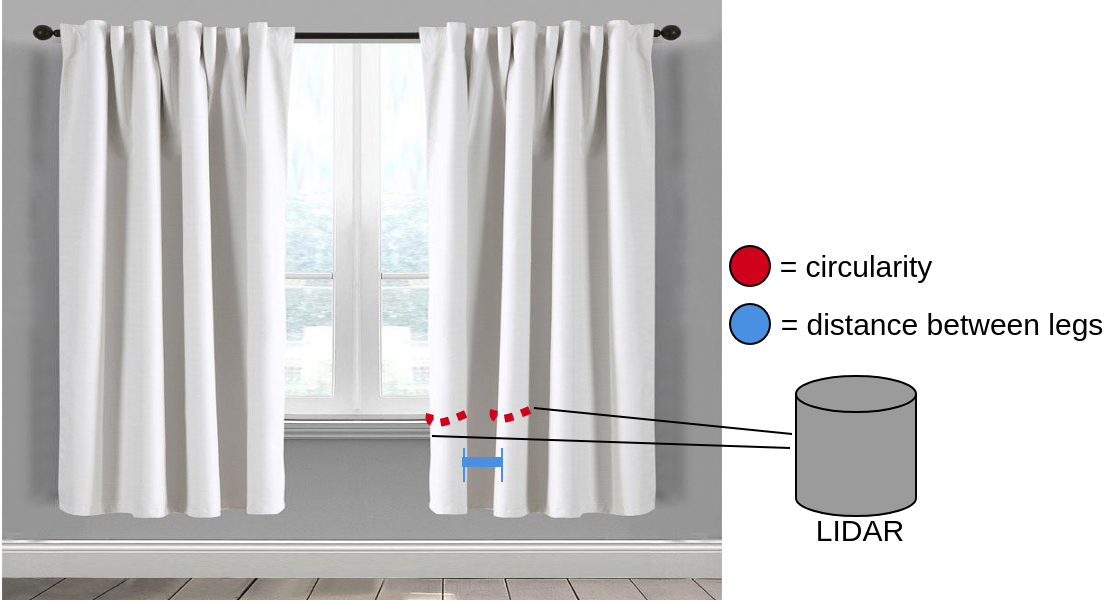
\includegraphics[width=1\textwidth]{figures/curtain.png} 
    \caption{This is a visual representation of how the LIDAR detects curtains as legs}
    \label{fig:curtains}
\end{figure}

Another thought is that, even though the cubes has been measured, the person standing inside them was not precisely measured towards the LIDAR itself, so the calculation of how far the LIDAR could reach would vary due to inaccuraccy of the measurement towards the LIDAR. However this was quickly noticed and is why the project commenced the test %(skriv om LIDAR testen).
\\
When the project tells the guiding robot to cancel its goal when the person it is guiding is not in the FOV anymore is a major further improvement since the LIDAR will not detect the person when the person is standing with the side to the robot. This means that every time the costumer will position itself to side when reaching or searching for a ware, the robot will then restart and all the inputted wares will be reset and the person will have to start all over. A way to distinguish this faulty manoeuvre is to place a RFID chip on the person using the robot. With this chip the robot will always recognise the person and only stop guiding and servicing the costumer when explicitly told to do so. This means that the costumer has to press on a button that stops the guiding bot and then it will be resat and another costumer can utilise its features and service. 

\section{Velocity control}

The velocity tests strive to keep the distancing in the social zone, as described in chapter \ref{ch:HRI} about HRI. However, when this was tested the robot's actual velocity did not even exceed a velocity of 0.5m/s, while the expected result were 0.7m/s. This will cause the robot to fall into the intimate zone depending on the person's velocity. The average pedestrian walks 1.2m/s according to the article from "geroscience" \cite{callisaya2017cognitive}. But considering the average pedestrian usually wants to get from A to B in a quick manner the walking speed could in theory be reduced even more. However, 0.430 as a maximum actual velocity is way to low even for a relaxed person strolling and looking at items in the shop. This concludes that another robot should have been used, since the turtlebot's maximum velocity, without payload, is 0.7m/s as described in chapter \ref{ch:equipment} describing the equipment. As stated in the actual test the overload of different equipment attached to the robot could have corrupted the max velocity, however this should not matter too much since the robots velocity is not close to the expected walking velocity of the average pedestrian.\\
The test was quite simple and could have been executed in a manner where a person was walking behind it and the robot should keep the expected distance at all time. However, as stated before, the turtlebot is very slow and the person's walking speed would have exceeded the turtlebot. If a robot with higher velocity was used in the project this test could have been realised.\\
To be more precise with the time measurements, better equipment should have been used, since chalk lines and mobile-phone recording of the time is not exactly the most sufficient method of recording the meters moved in seconds. The optimal setup would have been a laser pointer, much like a laser fence to detect whenever the robot would enter the desired zone and break the laser line when finishing, see fig \ref{fig:laserScan} for an idea of what is meant with laser lines and \ref{fig:velset} for the optimal setup of the velocity test.
\begin{figure}[H]
    \centering
    \begin{minipage}[b]{0.48\linewidth}
    \centering
    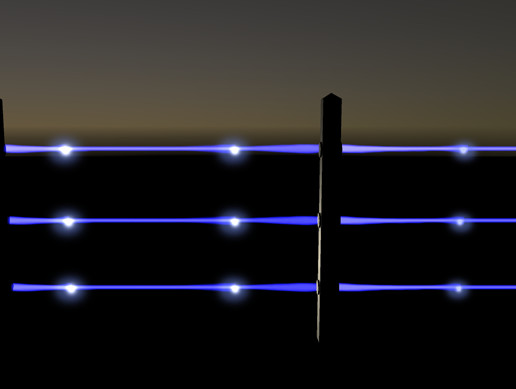
\includegraphics[width=\textwidth]{figures/laser.jpg}
    \caption{A visual representation of how the the laser fence should look at each end of the start and stop goals for the velocity test.}
    \label{fig:laserScan}
    \end{minipage}
    \hspace{0.2cm}
    \begin{minipage}[b]{0.48\linewidth}
    \centering
    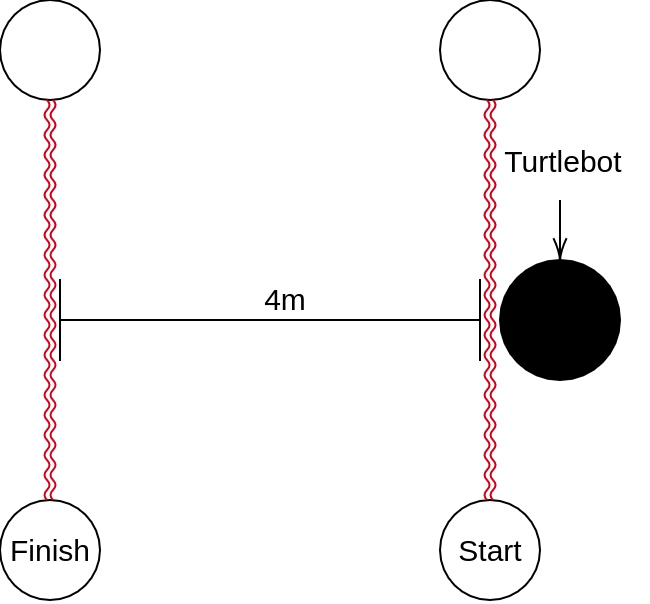
\includegraphics[width=\textwidth]{figures/veltest1.png}
    \caption{An automatised setup for the velocity test, making measurements more precise. The red wavy lines represents lasers.}
    \label{fig:velset}    
    \end{minipage}
\end{figure}

\section{State of the final prototype}
Some comments about the current state of the product. Is it good, is it bad, what would it need done to become good bla bla
\section{Further improvements}
After having discussed the current state of the robot, further improvements is a free space to talk about all the cool stuff time didn't allow, for example how thorough testing can reveal unknown information about the system and allow for developing a better product, if there was time left to do this.
